%&pdflatex
\RequirePackage{fix-cm}
\documentclass[smallextended]{svjour3} % svjour3: smallextended, referee
\usepackage[russian, english]{babel} % only english
\usepackage[T2A,T1]{fontenc} % only T1
\usepackage{graphicx}
\usepackage{amssymb, amsmath}
\allowdisplaybreaks[3]
\usepackage{cite}
\usepackage{fixltx2e}
\usepackage{fullpage}
\usepackage[export]{adjustbox}
\usepackage[skip=0pt]{subcaption}
\captionsetup{compatibility=false}

\usepackage{ifdraft}
\ifdraft{\renewcommand{\includegraphics}{\relax}}{\relax}
%\renewcommand{\includegraphics}{\relax}

\newcommand{\Kn}{\mathrm{Kn}}
\newcommand{\NS}{N\!S}
\newcommand{\dd}{\mathrm{d}}
\newcommand{\der}[2][]{\frac{\dd#1}{\dd#2}}
\newcommand{\pder}[2][]{\frac{\partial#1}{\partial#2}}
\newcommand{\pderdual}[2][]{\frac{\partial^2#1}{\partial#2^2}}
\newcommand{\pderder}[3][]{\frac{\partial^2#1}{\partial#2\partial#3}}
\newcommand{\Pder}[2][]{\partial#1/\partial#2}
\newcommand{\dzeta}{\boldsymbol{\dd\zeta}}
\newcommand{\bzeta}{\boldsymbol{\zeta}}
\newcommand{\Nu}{\mathcal{N}}
\newcommand{\Set}[2]{\{\,{#1}:{#2}\,\}}

%%% for the appendix
\newcommand{\B}{\ensuremath{\mathcal{B}^{(4)}}}
\newcommand{\Q}{\ensuremath{\mathcal{Q}^{(0)}}}
\newcommand{\T}[1]{\ensuremath{\mathcal{T}^{(#1)}}}
\newcommand{\TT}{\ensuremath{\tilde{\mathcal{T}}^{(0)}}}
\newcommand{\QQ}{\ensuremath{\tilde{\mathcal{Q}}^{(0)}}}
\newcommand{\ZD}[2]{\zeta_{#1}\delta_{#2}}
\newcommand{\ZZD}[3]{\zeta_{#1}\zeta_{#2}\delta_{#3}}
\newcommand{\ZZZ}{\zeta_i\zeta_j\zeta_k}
\newcommand{\ZZZZ}{\zeta_i\zeta_j\zeta_k\zeta_l}
\newcommand{\DD}[2]{\delta_{#1}\delta_{#2}}


\journalname{To be specified...}

\begin{document}

\title{
    Numerical analysis of the nonlinear plane Couette-flow problem for hard-sphere molecules
}

\author{O.A.~Rogozin}
\institute{O.A.~Rogozin \at
    Moscow Institute of Physics and Technology,
    9 Institutskiy pereulok, g. Dolgoprudny,
    Moskovskaya obl., Russian Federation\\
    \email{oleg.rogozin@phystech.edu}
}

\date{Received: date / Accepted: date}

\maketitle

\begin{abstract}
    The plane Couette flow of a rarefied gas is investigated on the basis of
    the Boltzmann equation for hard-sphere molecules.
    The velocity distribution function as well as its first thirteen moments is obtained from
    the accurate numerical solution based on the projection discrete-velocity method
    of evaluation of the collision integral, recently extended for nonuniform velocity grids~\cite{Dodulad2015}.
    The DSMC simulation is used to verify the obtained results over the wide range of the Knudsen and Mach numbers.
    The asymptotic solution for a slightly rarefied gas is also included in the comparison.
    Some transport coefficients for hard-sphere molecules are evaluated for this purpose.
    \keywords{
    	Couette flow \and
        rarefied gas dynamics \and
        Boltzmann equation \and
        projection method  \and
        asymptotic analysis \and
        OpenFOAM \and
        DSMC
    }
    \PACS{
        47.45.Ab,   % Kinetic theory of gases
        47.11.Df    % Finite volume methods
        47.15.-x    % Laminar flows
        51.10.+y    % Kinetic and transport theory of gases
    }
\end{abstract}

\section{Introduction}

%%% Linear problem
A stationary behavior of a gas between two parallel plates with the same temperature
and opposite velocities is one of the most fundamental boundary-value problems.
As for a rarefied gas, described on the basis of the Boltzmann equation,
the linearized Couette-flow problem has a long history of approximate methods~\cite{Willis1962}
and has been solved with good accuracy for hard-sphere molecules~\cite{Ohwada1990}.
The latter solution is often used for validation of other numerical methods~\cite{Fan2001,Aidun2010}.

%%% Nonlinear problem
The nonlinear problem is also studied extensively~\cite{Garzo2003}.
Despite the remarkable progress in deterministic numerical methods
in the recent years~\cite{Dimarco2014,Mieussens2014},
which can provide a high accuracy solution compared to stochastic techniques,
it is the DSMC simulation, with its inherent statistical fluctuations,
that remains as the reference solution~\cite{Cercignani1994}.
The present study is aimed to obtain the robust and accurate solution
of the nonlinear problem for various external parameters.

%%% The primary numeric method
The projection-interpolation method of discrete velocities is chosen for
evaluation of the Boltzmann integral~\cite{Tcheremissine1998, Tcheremissine2006}.
With this technique, velocities after impact that do not hit the grid
are projected to the adjacent grid points in such a way to conserve mass, momentum and energy.
The gain term of the Boltzmann integral is interpolated in such a way that
the discrete collision operator from the Maxwell distribution is strictly equal to zero.
Despite the fact that this algorithm of evaluation of the collision integral
provides the second order approximation~\cite{Anikin2012},
there are discontinuities of the distribution function in real boundary-value problems.
Therefore, nonuniform velocity grids, condensing in areas of large variation
of the distribution function, should be used.
For uniform grids, two projection points are enough to satisfy the conservation laws,
otherwise it is necessary to resort to the multipoint projection stencils~\cite{Dodulad2012}.
An extension of the projection method for nonuniform grids is represented in~\cite{Dodulad2015}.
It appears to the author that the proposed method can yield the most accurate results
among the existing numerical methods for the problem in question.

%%% Asymptotic solution
Fluid-dynamic-type equations are often used as an asymptotic solution for small Knudsen numbers.
The Navier--Stokes equations with the slip boundary conditions~\cite{Ohwada1989a}
provide an opportunity to construct the simplest solution~\cite{Sharipov2000}.
To take into account the next order of gas rarefaction, the Burnett equations can be considered~\cite{Reese2003}.
The rigorous asymptotic analysis of the Boltzmann equation,
based on the Hilbert expansion and systematic examination of the viscous boundary layer,
for arbitrary Mach numbers has been carried out in~\cite{Sone2000}.
Up to the first order of the Knudsen number, it also leads to the Navier-Stokes equations for the Couette-flow problem,
but some new transport coefficients are required to obtain the heat-flow vector and stress tensor.

\section{Formulation of the problem}

Consider a monatomic ideal gas between two infinite parallel plates with complete diffuse reflection.
A plane Couette flow is formed by relative motion of the plates relative to each other
with the longitudinal velocity (along the \(x\) axis),
while their temperatures remains constant.
The \(y\) axis is normal to the plates separated by distance \(L\).

In the present paper we deal with dimensionless quantities, so the macroscopic variables
have the following form: \(p_{ij}p^{(0)}\) is the stress tensor, \(TT^{(0)}\) is the temperature,
\(\rho p^{(0)}/RT^{(0)}\) is the density, \(v_i(2RT^{(0)})^{1/2}\) is the velocity
and \(q_ip^{(0)}(2RT^{(0)})^{1/2}\) is the heat-flow vector.
The specific gas constant \(R = k_B/m\), where \(k_B\) is the Boltzmann constant
and \(m\) is the molar mass.
Let \(L\) be a unit of length and the velocities of the plates (\(y=\pm1/2\))
be equal to \((\pm\Delta{v}/2)(2RT^{(0)})^{1/2}\), respectively.
\(T^{(0)}\) is the common temperature of the plates.
\(p^{(0)}\) is selected in such a way that the average density is equal to one, i.e.,
\begin{equation}\label{eq:total_mass}
    \int_{-\frac12}^\frac12\rho\dd{y} = 1.
\end{equation}

\subsection{Kinetic description}

Molecules are assumed as hard spheres, so the Knudsen number is expressed in the following way:
\begin{equation}\label{eq:Kn_number}
    \Kn = \frac{\ell_0}{L} = \frac{k_BT^{(0)}}{\pi\sqrt{2} d_m^2p^{(0)}L},
\end{equation}
where \(\ell_0\) is the mean free path for the unit density, \(d_m\) is the diameter of the molecule.
To describe an ideal gas over the wide range of Knudsen numbers
we should turn to the Boltzmann equation.
Its dimensionless and time-independent form is as follows:
\begin{equation}\label{eq:Boltzmann}
    \zeta_i\pder[f]{x_i} = \frac1k J(f,f),
\end{equation}
where the collision integral
\begin{equation}\label{eq:ci}
    J(f,g) = \frac12 \int (f'g'_* + f'_*g' - fg_* - f_*g) B
    \dd \Omega(\boldsymbol{\alpha}) \dzeta_*,
\end{equation}
is taken from the distribution function \(f(x_i,\zeta_i)(2p^{(0)})/(2RT^{(0)})^{5/2}\)
in space \((x_iL, \zeta_i(2RT^{(0)})^{1/2})\).
\(\dd \Omega(\boldsymbol{\alpha})\) is an element of solid angle in the direction of the unit vector \(\alpha_i\),
determining the velocities after impact:
\begin{equation}\label{eq:after_impact}
    \zeta'_i = \zeta_i + \alpha_i\alpha_j(\zeta_{j*}-\zeta_j), \quad
    \zeta'_{i*} = \zeta_{i*} - \alpha_i\alpha_j(\zeta_{j*}-\zeta_j).
\end{equation}
For the hard-sphere model,
\begin{equation}\label{eq:ci_kernel}
    B = \frac{|\alpha_i(\zeta_{i*}-\zeta_i)|}{4\sqrt{2\pi}}.
\end{equation}
A modified Knudsen number \(k = \Kn\sqrt\pi/2\) is used in~\eqref{eq:Boltzmann}.

The Maxwell-type boundary condition with diffuse reflection is used at \(y=1/2\), i.e.,
\begin{equation}\label{eq:diffuse_bc}
    f(\zeta_x,\zeta_y,\zeta_z) = \frac2\pi \exp\left[-\left(\zeta_x-\frac{\Delta{v}}{2}\right)^2-\zeta_y^2-\zeta_z^2\right]
        \int_{\zeta_{*y}>0}\zeta_{*y} f_* \dzeta_*, \quad \zeta_y<0.
\end{equation}
The symmetry condition is imposed at \(y=0\):
\begin{equation}\label{eq:diffuse_bc}
    f(\zeta_x,\zeta_y,\zeta_z) = f(\zeta_x,-\zeta_y,\zeta_z), \quad \zeta_y>0.
\end{equation}

The nondimensional macroscopic variables are calculated by integrating the distribution function:
\begin{equation}\label{eq:macro}
    \begin{gathered}
    \rho = \int f \dzeta, \quad
    v_i = \frac1{\rho} \int \zeta_i f \dzeta, \\
    T = \frac{2}{3\rho}\int(\zeta_i-v_i)^2 f \dzeta, \quad
    q_i = \int(\zeta_i-v_i)(\zeta_j-v_j)^2 f \dzeta, \\
    p_{ij} = 2 \int(\zeta_i-v_i)(\zeta_j-v_j) f \dzeta,
        \quad p = p_{ii}/3 = \rho T.
    \end{gathered}
\end{equation}

\subsection{Linearization of the problem}

Linearized Boltzmann equation
\begin{equation}\label{eq:linear_Boltzmann}
    \zeta_i \pder[\phi]{x_i} = \frac1k \mathcal{L}(\phi),
\end{equation}
with the linearized collision operator
\begin{equation}\label{eq:linear_ci}
    \mathcal{L}(\phi) = \int E_*(\phi'+\phi'_*-\phi-\phi_*) B
    \dd \Omega(\boldsymbol{\alpha}) \dzeta_*
\end{equation}
holds for a gas that deviates only slightly from an equilibrium state, i.e.,
\begin{equation}\label{eq:linear_condition}
    \phi = \frac{f}{E} - 1 \ll 1, \quad E(\zeta) = \frac1{\pi^{3/2}}\exp\left(-\zeta^2\right).
\end{equation}
Perturbed local Maxwell distribution
\begin{equation}\label{eq:linear_maxwellian}
    \phi_e = \omega + 2\zeta_i v_i + \left(\zeta_i^2-\frac32\right)\tau
\end{equation}
is expressed in terms of the corresponding perturbed macroscopic variables:
\begin{equation}
    \omega = \rho-1, \quad \tau = T-1, \quad P = p-1, \quad P_{ij} = p_{ij}-\delta_{ij},
\end{equation}
where \(\delta_{ij}\) is the Kronecker delta function

In particular, the Couette-flow problem is linearized when \(\Delta{v}\ll 1\).
Then the distribution function can be expressed in the following form:
\begin{equation}\label{eq:linear_solution}
    \phi = \Delta{v} \zeta_x \Phi(y,\zeta_y,\zeta), \quad \zeta = \sqrt{\zeta_i^2},
\end{equation}
Substituting~\eqref{eq:linear_solution} into~\eqref{eq:linear_Boltzmann}, we obtain
\begin{equation}\label{eq:linear_equation}
    \zeta_y \pder[\Phi]{y} = \frac1{k\zeta_x}\mathcal{L}(\zeta_x\Phi)
\end{equation}
with the following boundary conditions:
\begin{equation}\label{eq:linear_bc}
    \Phi_-(1/2,\zeta_y,\zeta) = 1, \quad \Phi_+(0,\zeta_y,\zeta) = -\Phi_-(0,-\zeta_y,\zeta),
\end{equation}
where \(\Phi_\pm = \Phi(\zeta_y \gtrless 0)\).
Thus, the perturbed macroscopic variables take the following form:
\begin{equation}\label{eq:linear_macro}
    \frac{P_{xy}}{\Delta{v}} = 2\int \zeta_x^2 \zeta_y \Phi E\dzeta, \quad
    \frac{v_x}{\Delta{v}} = \int \zeta_x^2 \Phi E\dzeta, \quad
    \frac{q_x}{\Delta{v}} = \int \zeta_x^2 \zeta^2 \Phi E\dzeta - \frac52 \frac{v_x}{\Delta{v}}.
\end{equation}
Other variables from~\eqref{eq:macro} remain constant in the linear case.

\section{Outline of the methods for the linear problem}

For \(k\to\infty\), we obtain the collisionless linearized Boltzmann equation \(\zeta_y\Pder[\Phi]{y} = 0\),
which has a simple solution as a combination of two different half-Maxwellians, i.e., \(\Phi_\pm = \mp 1\).
It gives
\begin{gather}\label{eq:linear_free_macro}
    \frac{P_{xy}}{\Delta{v}} = -\frac1{\sqrt\pi}, \quad v_x = q_x = 0.
\end{gather}

For small \(k\), we turn to the Grad--Hilbert expansion
that gives the following asymptotic solution~\cite{Sone2007}:
\begin{equation}\label{eq:small_solution}
    \Phi = \frac{2y - \zeta_y \mathcal{B}(\zeta) k}{1-2k_0k},
\end{equation}
where special function \(\mathcal{B}(\zeta)\) is defined from the integral equation
\begin{equation}\label{eq:transport_B}
    \mathcal{L}\left[\left(\zeta_i\zeta_j-\frac{\zeta^2}3\delta_{ij}\right) \mathcal{B}(\zeta)\right]
        = -2 \left(\zeta_i\zeta_j-\frac{\zeta^2}3\delta_{ij}\right).
\end{equation}
The solution~\eqref{eq:small_solution} does not satisfy the boundary conditions~\eqref{eq:linear_bc},
therefore, it is corrected in the Knudsen layer. Finally, we have
\begin{equation}\label{eq:small_macro}
    \frac{P_{xy}}{\Delta{v}} = - \frac{\gamma_1 k}{1-2k_0k}, \quad
    \frac{v_x}{\Delta{v}} = \frac{y - (Y_0^--Y_0^+)k}{1-2k_0k}, \quad
    \frac{q_x}{\Delta{v}} = \frac{(H_A^--H_A^+)k}{1-2k_0k},
\end{equation}
where the viscosity coefficient \(\gamma_1 = 1.270042427\) is calculated as
\begin{equation}\label{eq:gamma_1}
    \gamma_1 = \frac{8}{15\sqrt\pi}\int_0^\infty \zeta^6 \mathcal{B}(\zeta)E\dd\zeta,
\end{equation}
and \(k_0 = -1.2540\) is the slip coefficient.
The Knudsen-layer functions \(K^\pm = Y_0^\pm, H_A^\pm\) are defined as follows:
\begin{equation}\label{eq:linear_knudsen_functions}
     K^\pm = K(\eta_\pm), \quad \eta_\pm = \frac{1 \mp 2y}{2k}.
\end{equation}
For hard-sphere molecules, \(Y_0(\eta)\), \(H_A(\eta)\)
are tabulated in~\cite{Ohwada1989a, Sone2002, Sone2007}.

In case of arbitrary \(k\), the solution can be obtained by numerical analysis.
For example, it has been carefully accomplished in~\cite{Ohwada1990} for the hard-sphere model.

For comparison, we also consider a solution of the widely used BKW (Boltzmann--Krook--Welander) equation,
whose linearized form of collision integral
\begin{equation}\label{eq:linear_bkw}
    \mathcal{L}(\phi) = -\phi + \omega + 2\zeta_i v_i + \left(\zeta_i^2-\frac32\right)\tau
\end{equation}
leads to the differential equation
\begin{equation}\label{eq:linear_bkw_equation}
    \zeta_y \pder[\Phi]{y} = \frac1{k}\left( \frac{2v_x}{\Delta{v}} - \Phi \right).
\end{equation}
Its solution can be written in the following form~\cite{Willis1962}:
\begin{equation}\label{eq:bkw_solution}
    \Phi_\pm = \mp \exp\left(\mp\frac{\eta_\mp}{\zeta_y}\right) +
        \int_{\mp\frac12}^y \frac1{k\zeta_y} \exp \left(-\frac{y-s}{k\zeta_y}\right) g(s) \dd{s},
\end{equation}
where \(g(y) = 2v_x/\Delta v\) is found from the Fredholm integral equation of the second kind
\begin{equation}\label{eq:bkw_g_equation}
    \sqrt\pi g(y) = \mathcal{T}_0^+ - \mathcal{T}_0^-
        + \frac1k \int_0^{\frac12} \left[ \mathcal{T}_{-1}\left(\frac{|y-s|}{k}\right)
        - \mathcal{T}_{-1}\left(\frac{y+s}{k}\right) \right] g(s) \dd{s}.
\end{equation}
Here, \(\mathcal{T}_n(s)\) are special Abramowitz functions~\cite{Abramowitz1972}:
\begin{equation}\label{eq:Abramowitz}
    \mathcal{T}_n(s) = \int_0^\infty t^n \exp\left(-t^2-\frac{s}{t}\right) \dd t,
    \quad s\ge0, \quad n \in \mathbb{Z}.
\end{equation}
The remaining macroscopic variables are calculated as follows:
\begin{gather}
    \frac{P_{xy}}{\Delta v} = -\frac{2k}{\sqrt\pi} \left(
        \mathcal{T}_2(0)-\mathcal{T}_2\left(\frac1k\right)
        + \frac1k\int_0^{\frac12}\left[
            \mathcal{T}_1\left(\frac{1-2s}{2k}\right)-\mathcal{T}_1\left(\frac{1+2s}{2k}\right)
        \right]g(s)\dd{s}
        \right), \label{eq:bkw_macro_Pxy} \\
    \frac{q_x}{\Delta v} = \frac1{2\sqrt\pi}\left(
        \mathcal{T}_2\left(\frac{1-2s}{2k}\right) - \mathcal{T}_2\left(\frac{1+2s}{2k}\right)
        + \frac1k\int_0^{\frac12}\left[
            \mathcal{T}_1\left(\frac{|y-s|}k\right)-\mathcal{T}_1\left(\frac{y+s}k\right)
        \right]g(s)\dd{s}
        \right) - \frac{g(y)}4. \label{eq:bkw_macro_qx}
\end{gather}

\section{Outline of the methods for the nonlinear problem}

\subsection{Free molecular solution}

Collisionless Boltzmann equation, as well as in the linearized case,
has a solution as a combination of two different half-Maxwellians:
\begin{equation}\label{eq:free_solution}
    f^\pm = f(\zeta_y \gtrless 0) =
        \frac1{\pi\sqrt\pi} \exp\left[-\left(\zeta_x\pm\frac{\Delta{v}}2\right)^2 - \zeta_y^2 - \zeta_z^2\right],
\end{equation}
which supplements Eqs.~\eqref{eq:linear_free_macro} with the following values of the macroscopic variables:
\begin{equation}\label{eq:free_macro}
    \frac{\tau}{(\Delta{v})^2} = \frac16, \quad q_y = 0, \quad
    \frac{P_{xx}}{(\Delta{v})^2} = \frac12, \quad P_{yy} = P_{zz} = 0.
\end{equation}

\subsection{Navier--Stokes equations}\label{sec:Navier-Stokes}

The equations of conservation of momentum and energy for the Couette-flow problem
degenerate into the following dimensionless form:
\begin{equation}\label{eq:conservation_laws}
    \pder[p]{y} = 0, \quad \pder[p_{xy}]{y} = 0, \quad \pder{y}(v_x p_{xy} + q_y) = 0.
\end{equation}
Substituting Newton's and Fourier's laws
\begin{equation}\label{eq:Newton-Fourier}
    p_{xy} = -\gamma_1 k\sqrt{T}\pder[v_x]{y}, \quad q_y = -\frac54\gamma_2 k\sqrt{T}\pder[T]{y}
\end{equation}
into Eqs.~\eqref{eq:conservation_laws}, we obtain a system of differential equations
\begin{equation}\label{eq:Navier-Stokes}
    \pder{y}\left(\sqrt{T}\pder[v_x]{y}\right) = 0, \quad
    \sqrt{T}\left(\pder[v_x]{y}\right)^2 + \frac54\frac{\gamma_2}{\gamma_1}\pder{y}\left(\sqrt{T}\pder[T]{y}\right) = 0,
\end{equation}
which can be solved with the nonslip boundary conditions at \(y=1/2\):
\begin{equation}\label{eq:nonslip_bc}
    v_x = \frac{\Delta{v}}2, \quad T = 1.
\end{equation}
Incidentally, \(\gamma_2 = 1.922284066\) is the thermal conductivity coefficient.
The constant pressure \(p\) is calculated from the total mass of the gas (see~\eqref{eq:total_mass}):
\begin{equation}\label{eq:constant_pressure}
    p = \left( 2\int_{0}^\frac12\frac{\dd{y}}{T} \right)^{-1}.
\end{equation}

\subsection{Asymptotic analysis for small Knudsen numbers}

The Navier--Stokes equations can be obtained from the Chapman--Enskog expansion
and, in essence, is a kind of disturbance of the equilibrium Maxwellian state.
To obtain a rigorous asymptotic solution for small \(k\),
we should refer to the Hilbert expansion in connection with viscous boundary and Knudsen layers.
A detailed algorithm for construction of such a solution for the boundary-value problem
is presented in~\cite{Sone2000, Sone2002}.

Expanding macroscopic variables \(h = \rho, v_i, T, \dots\) into a power series of \(k\), i.e.,
\begin{equation}\label{eq:hilbert_expansion}
    h = h_0 + h_1k + h_2k^2 + \cdots,
\end{equation}
we obtain, in the context of the plane Couette-flow problem, the following set of equations up to the first order:
\begin{gather}
    \pder{y}\left( \sqrt{T_0}\pder[v_{x0}]{y} \right) = 0, \label{eq:Hilbert_U0}\\
    \sqrt{T_0}\left( \pder[v_{x0}]{y}\right)^2 + \frac{5\gamma_2}{4\gamma_1}\pder{y}\left(\sqrt{T_0}\pder[T_0]{y} \right) = 0, \label{eq:Hilbert_T0}\\
    \pder{y}\left( \sqrt{T_0}\pder[v_{x1}]{y} + \frac{T_1}{2\sqrt{T_0}}\pder[v_{x0}]{y} \right) = 0, \label{eq:Hilbert_U1}\\
    \left( 2\sqrt{T_0}\pder[v_{x1}]{y} + \frac{T_1}{2\sqrt{T_0}}\pder[v_{x0}]{y} \right) \pder[v_{x0}]{y}
        + \frac{5\gamma_2}{4\gamma_1} \pder{y}\left( \sqrt{T_0}\pder[T_1]{y} + \frac{T_1}{2\sqrt{T_0}}\pder[T_0]{y} \right) = 0. \label{eq:Hilbert_T1}
\end{gather}
The leading-order equations~\eqref{eq:Hilbert_U0}--\eqref{eq:Hilbert_T0}
is seen to coincide with the Navier--Stokes equations~\eqref{eq:Navier-Stokes}.
The pressure is constant up to the first order:
\begin{equation}\label{eq:hilbert_pressure}
    \pder[p_0]{y} = 0, \quad \pder[p_1]{y} = 0.
\end{equation}

Boundary conditions at \(y=1/2\),
\begin{gather}
    v_{x0} = v_{Bx0}, \quad v_{x1} = v_{Bx1} + k_0 \frac{T_0}{p_0} \pder[v_{x0}]{y}, \label{eq:hilbert_bc_U}\\
    T_0 = T_{B0}, \quad T_1 = T_{B1} - d_1 \frac{T_0}{p_0} \pder[T_0]{y}, \label{eq:hilbert_bc_T}
\end{gather}
imply some freedom of the expansion in \(k\):
\begin{equation}\label{eq:hilbert_boundary_expansion}
    \frac{\Delta{v}}2 = v_{Bx} = v_{Bx0} + v_{Bx1}k, \quad 1 = T_B = T_{B0} + T_{B1}k.
\end{equation}
Putting \(T_1 = 0\) and \(v_{x1} = 0\) at \(y=1/2\), we obtain a trivial solution for~\eqref{eq:Hilbert_U1}--\eqref{eq:Hilbert_T1}:
\(T_1 = 0\) and \(v_{x1} = 0\). Thus, we come to the Navier--Stokes equations with the slip boundary conditions.

Taking into account the Knudsen-layer correction, the asymptotic solution takes the following form:
\begin{gather}
    p = \left( 2\int_{0}^\frac12\frac{\dd{y}}{T_0} \right)^{-1}
        - (\Omega_1^-+\Omega_1^+ + \Theta_1^-+\Theta_1^+)\left.\pder[T_0]{y}\right|_{y=\frac12}k, \label{eq:Hilbert_p}\\
    v_x = v_{x0} - \frac{Y_0^--Y_0^+}{p_0}T_{B0}\left.\pder[v_{x0}]{y}\right|_{y=\frac12}k, \label{eq:Hilbert_U}\\
    T = T_0 - \frac{\Theta_1^-+\Theta_1^+}{p_0}T_{B0}\left.\pder[T_0]{y}\right|_{y=\frac12}k, \label{eq:Hilbert_T}\\
    p_{xy} = -\gamma_1\sqrt{T_0}\pder[v_{x0}]{y}k, \label{eq:Hilbert_Pxy}\\
    q_x = (H_A^--H_A^+)T_{B0}\left.\pder[v_{x0}]{y}\right|_{y=\frac12}k + \frac{T_0}{p_0}\left(\frac{\gamma_3}2 T_0 \pderdual[v_{x0}]{y}
        + 4\gamma_{10} \pder[T_0]{y}\pder[v_{x0}]{y}\right)k^2, \label{eq:Hilbert_Qx}\\
    q_y = -\frac54\gamma_2\sqrt{T_0}\pder[T_0]{y}k, \label{eq:Hilbert_Qy}\\
    \begin{aligned}
    p_{xx} - p &= -\frac12 (\Omega_1^-+\Omega_1^+ + \Theta_1^-+\Theta_1^+)\left.\pder[T_0]{y}\right|_{y=\frac12}k \\
        &+ \frac1{3p_0}\left[-\left(\gamma_3 T_0 \pderdual[T_0]{y} + \gamma_7\left(\pder[T_0]{y}\right)^2\right)
        + 2(\gamma_8+\gamma_9)T_0\left(\pder[v_{x0}]{y}\right)^2\right]k^2,
    \end{aligned}\label{eq:Hilbert_Pxx}\\
    \begin{aligned}
    p_{yy} - p &= (\Omega_1^-+\Omega_1^+ + \Theta_1^-+\Theta_1^+)\left.\pder[T_0]{y}\right|_{y=\frac12}k \\
        &+ \frac1{3p_0}\left[2\left(\gamma_3 T_0 \pderdual[T_0]{y} + \gamma_7\left(\pder[T_0]{y}\right)^2\right)
        + 2(\gamma_8-2\gamma_9)T_0\left(\pder[v_{x0}]{y}\right)^2\right]k^2,
    \end{aligned}\label{eq:Hilbert_Pyy}\\
    \begin{aligned}
    p_{zz} - p &= -\frac12 (\Omega_1^-+\Omega_1^+ + \Theta_1^-+\Theta_1^+)\left.\pder[T_0]{y}\right|_{y=\frac12}k \\
        &+ \frac1{3p_0}\left[-\left(\gamma_3 T_0 \pderdual[T_0]{y} + \gamma_7\left(\pder[T_0]{y}\right)^2\right)
        + 2(\gamma_9-2\gamma_8)T_0\left(\pder[v_{x0}]{y}\right)^2\right]k^2,
    \end{aligned}\label{eq:Hilbert_Pzz}
\end{gather}
Here, the following thermal-stress transport coefficients are used:
\begin{equation}\label{eq:gamma_tabular}
    \gamma_3 = 1.947906335, \quad \gamma_7 = 0.189201.
\end{equation}
Evaluation of the transport coefficients \(\gamma_8\), \(\gamma_9\), \(\gamma_{10}\)
for the hard-sphere model are not presented in the literature (as far as the author is aware),
so they were obtained by direct solution of the corresponding integral equations
(see Appendix~\ref{sec:gamma_coeffs}):
\begin{equation}\label{eq:gamma_numerical}
    \gamma_8 = 1.496(3), \quad \gamma_9 = 1.635(7), \quad \gamma_{10} = 2.463(3).
\end{equation}
The Knudsen-layer functions \(K^\pm = Y_0^\pm, \Theta_1^\pm, H_A^\pm, \Omega_1^\pm\)
are defined as follows:
\begin{equation}\label{eq:linear_knudsen_functions}
     K^\pm = K(p_0\eta_\pm), \quad \eta_\pm = \frac{1 \mp 2y}{2k}.
\end{equation}
For hard-sphere molecules, \(\Theta_1(\eta)\) and \(\Omega_1(\eta)\)
are tabulated in~\cite{Ohwada1992, Sone2002, Sone2007}.
Note that the pressure \(p\) from~\eqref{eq:Hilbert_Pxx}--\eqref{eq:Hilbert_Pzz}
includes the nonuniform high-order term \(p_2\),
which is missed in~\eqref{eq:Hilbert_p}.

The presented set of equations~\eqref{eq:Hilbert_U0}--\eqref{eq:Hilbert_T0}
with the boundary conditions~\eqref{eq:hilbert_bc_U}--\eqref{eq:hilbert_bc_T}
is solved accurately by the finite-volume method
implemented in OpenFOAM\textregistered{}.

\subsection{Statistical simulation}

The DSMC method is the dominant numerical method in rarefied gas dynamics.
Its description is omitted in the present paper,
because it can be easily found in literature~\cite{Bird1994,Sone2007}.
An open-source parallel solver, \verb+dsmcFoam+~\cite{dsmcFoam2010},
based on the widespread CFD toolbox OpenFOAM\textregistered{}, is used.

Numerical simulation of gas between two parallel plates is carried out
in a two-dimensional geometry \((x,y)\) with a periodicity boundary conditions along the \(y\) axis.
The size of the statistical ensemble is \(2\cdot10^6\) for \(\Delta{v}=0.1\)
and \(2\cdot10^5\) for \(\Delta{v}\ge1\).
The space interval \(0<y<1/2\) is divided into uniform sections:
from 40 for \(\Kn=10\) to 100 for \(\Kn=0.1\).
The time step is chosen empirically to provide a satisfactory approximation of the macroscopic variables:
\begin{equation}\label{eq:dsmc_timestep}
    \Delta{t} = \frac\pi2 \frac{\sqrt\Kn}{1000}.
\end{equation}
The shear stress \(P_{xy}\) is the most sensitive variable to step \(\Delta{t}\).
The other quantities can be calculated with the same accuracy by a tenfold increase of the time step.
In order to reduce the statistical noise, values of all macroscopic variables
are averaged over time after reaching a steady state.

\subsection{Discrete-velocity solution}

The Boltzmann equation can be solved directly by symmetric splitting
into the advection equation
\begin{equation}\label{eq:split_advection}
    \pder[f]{t} + \zeta_i\pder[f]{x_i} = 0,
\end{equation}
for which a finite-volume method with an explicit second-order TVD scheme is used,
and the relaxation equation
\begin{equation}\label{eq:split_integral}
    \pder[f]{t} = \frac1k J(f,f),
\end{equation}
for which the projection-interpolation method of discrete velocities
on nonuniform grids is used~\cite{Dodulad2015}.
Below we outline only the conservative technique for evaluation
of the Boltzmann collision integral, which is the crucial point of the overall method.

%%% Numerical approximation
Let a regular velocity grid be constructed so that
the cubature in \(\bzeta\) space is expressed in the weighted sum
\begin{equation}\label{eq:zeta_cubature}
    \int F(\bzeta) \dzeta \approx \sum_{\gamma\in\Gamma} F_\gamma w_\gamma,
        \quad \sum_{\gamma\in\Gamma} w_\gamma = V_\nu,
        \quad F_\gamma = F(\bzeta_\gamma),
\end{equation}
where \(\mathcal{V} = \Set{\zeta_\gamma}{\gamma\in\Gamma}\) is the set of the integration points,
\(F\) is an arbitrary function of \(\bzeta\),
\(V_\nu\) is the total volume of the velocity grid.
Then, the collision integral written in the symmetrized form,
\begin{equation}\label{eq:symm_ci}
    J(f_\gamma, f_\gamma) = \frac14\int \left[
        \delta(\bzeta'-\bzeta_\gamma) + \delta(\bzeta'_*-\bzeta_\gamma)
        - \delta(\bzeta-\bzeta_\gamma) - \delta(\bzeta_*-\bzeta_\gamma)
        \right](f'f'_* - ff_*)B \dd\Omega(\boldsymbol{\alpha}) \dzeta\dzeta_*,
\end{equation}
where \(\delta(\bzeta)\) is the Dirac delta function in \(\mathbb{R}^3\),
has the following discrete analog:
\begin{equation}\label{eq:discrete_symm_ci}
    w_\gamma J_\gamma = \frac{\pi V_\nu^2}{\sum_{\nu\in\Nu} w_{\alpha_\nu}w_{\beta_\nu}}
        \sum_{\nu\in\Nu} \left(
            \delta_{\alpha'_\nu\gamma} + \delta_{\beta'_\nu\gamma}
            - \delta_{\alpha_\nu\gamma} - \delta_{\beta_\nu\gamma}
        \right)\left(
            \frac{w_{\alpha_\nu}w_{\beta_\nu}}{w_{\alpha'_\nu}w_{\beta'_\nu}}
            \hat{f}_{\alpha'_\nu}\hat{f}_{\beta'_\nu} - \hat{f}_{\alpha_\nu}\hat{f}_{\beta_\nu}
        \right)B_\nu,
\end{equation}
Here, \(\alpha_\nu\in\Gamma\) and \(\beta_\nu\in\Gamma\), along with \(\boldsymbol{\alpha}_\nu\),
are taken from the Korobov's lattice rule~\cite{Korobov1959,Dick2013}
for the eight-dimensional cubature.
In addition, the integration lattice is randomly shifted every time step.
The modified distribution function \(\hat{f}_\gamma = f_\gamma w_\gamma\) is used for convenient.
To satisfy~\eqref{eq:total_mass} exactly, the following approximation of the Maxwell distribution is used:
\begin{equation}\label{eq:discrete_Maxwell}
    \hat{f}_{M\gamma} = \rho\left[\sum_{\alpha\in\Gamma}w_\alpha\exp
            \left(-\frac{\bzeta_\alpha - \boldsymbol{v}}{T}\right)
        \right]^{-1}
        w_\gamma\exp\left(-\frac{\bzeta_\gamma - \boldsymbol{v}}{T}\right).
\end{equation}

%%% Projection and interpolation
In the general case, the velocities after impact,
\(\bzeta_{\alpha'_\nu}\) and \(\bzeta_{\beta'_\nu}\), are not in \(\mathcal{V}\).
If they are just replaced with the nearest grid velocities,
\(\bzeta_{\lambda_\nu}\in\mathcal{V}\) and \(\bzeta_{\mu_\nu}\in\mathcal{V}\),
the discrete collision integral~\eqref{eq:discrete_symm_ci} is no longer strictly conservative.
Moreover, the discrete Maxwell distribution is no longer the equilibrium state.
Therefore, the following two procedures are applied in the projection-interpolation method.
First, \(\bzeta_{\alpha'_\nu}\) is projected to \(\bzeta_{\lambda_\nu}\) and
some adjacent grid points, \(\Set{\bzeta_{\lambda_\nu+s_a}}{a\in\Lambda}\subset\mathcal{V}\),
in the following way:
\begin{equation}\label{eq:ci_projection}
    \delta_{\alpha'_\nu\gamma} = \sum_{a\in\Lambda} r_{\lambda,a}\delta_{\lambda_\nu+s_a,\gamma}.
\end{equation}
The weights \(r_{\lambda,a}\) are selected to provide the conservation of mass, momentum and energy, i.e.,
\begin{equation}\label{eq:impact_conservation}
    \sum_{a\in\Lambda} r_{\lambda,a} = 1, \quad
    \sum_{a\in\Lambda} r_{\lambda,a} \bzeta_{\lambda_\nu+s_a} = \bzeta_{\alpha'_\nu}, \quad
    \sum_{a\in\Lambda} r_{\lambda,a} \bzeta_{\lambda_\nu+s_a}^2 = \bzeta_{\alpha'_\nu}^2.
\end{equation}
The set of projection points \(\mathcal{S}_{\alpha'_\nu} = \Set{\bzeta_{\lambda_\nu+s_a}}{a\in\Lambda, r_{\lambda,a}\neq0}\)
is called the projection stencil.
In the present paper, the minimal stencil for a nonuniform velocity grid is used, \(|\mathcal{S}_{\alpha'_\nu}|=5\).
Second, to satisfy \(J_\gamma(\hat{f}_{M\gamma}, \hat{f}_{M\gamma}) = 0\),
\(\hat{f}_{\alpha'_\nu}\) is interpolated in following way:
\begin{equation}\label{eq:ci_interpolation}
    \frac{\hat{f}_{\alpha'_\nu}}{w_{\alpha'_\nu}} = \prod_{a\in\Lambda}
        \left(\frac{\hat{f}_{\lambda_\nu+s_a}}{w_{\lambda_\nu+s_a}} \right)^{r_{\lambda,a}}.
\end{equation}
For \(\bzeta_{\beta'_\nu}\) and \(\hat{f}_{\beta'_\nu}\), all formulas are similar.

\subsubsection{Discretization of the problem}

%%% The grid in the velocity
The discrete velocity space is bounded by the prolate spheroid
filled with the centered rectangular grid \(\mathcal{V}\).
The symmetry axis of the spheroid is parallel to \(x\) axis.
\(\zeta^{(\mathrm{cut})}_x\) is the semi-major axis, \(\zeta^{(\mathrm{cut})}_r\) is the semi-minor axis.
For the Couette-flow problem, the distribution function is sufficiently smooth along \(\zeta_x\) and \(\zeta_z\).
In addition, in the entire domain occupied by the gas, \(\zeta_z\) component of the distribution
differs slightly from the Maxwellian with \(v_z=0\).
Therefore, \(\zeta_z\) coordinates of \(\bzeta_\gamma\) are selected as the roots of the Hermite polynomials,
since the Gauss--Hermite quadrature is known to provide the maximum order of approximation
to evaluate integrals of the form \(\int h(s)\exp(-s^2)\dd{s}\).
Along \(\zeta_x\) axis, the distance between points is constant.
\(\zeta_y\) coordinates of \(\bzeta_\gamma\) are drift apart from \(\zeta_y=0\)
as a geometric sequence with the ratio \(r\).
It allows significant variations of the distribution function near \(\zeta_y=0\) to be approximated more accurately.
The weights \(w_\gamma\) are selected to provide a midpoint approximation in~\eqref{eq:zeta_cubature}.

%%% The grid in the physical space
The physical volume of the problem (\(0<y<1/2\)) consists of \(N_x\) cells arranged in a single row.
For small \(\Kn\), the physical grid should be refined near \(y=1/2\)
due to significant variations of the solution in the thin Knudsen layer in comparison to the overall volume.
%%% Remark on a time step
Owing to the CFL condition for convergence of an explicit scheme for~\eqref{eq:split_advection},
the time step is of the same order as the size of the marginal cell.
Therefore, to accelerate progress towards the steady state for small \(\Kn\),
the initial distribution function is constructed as the local Maxwellian
with \(\rho\), \(v_i\), and \(T\) obtained from the simulation on the coarse uniform grid.
Moreover, the solution for the smallest \(\Kn\) does not reach the steady state completely.
The iteration is stopped when the amplitude of time variations reduces to about \(10^{-4}\).

\subsubsection{Control of accuracy}

The physical grid is refined in such a way
that the width of the marginal cell is about \(\Kn/100\).
This condition provides an accuracy of the order of \(10^{-4}\) for the trapezoidal-rule quadrature
of the Knudsen-layer functions like \(Y_0(\eta)\), \(H_A(\eta)\).
For \(\Kn=100\), when the solution is similar to the constant over the physical space,
\(N_x = 30\) is sufficient for the same precision.

To assess the accuracy of the discrete approximation in \(\zeta_i\) space,
two outermost models of the distribution function were considered.
For small \(\Kn\), this is a Grad's thirteen-moment approximation
\begin{equation}\label{eq:grad13}
    f = \frac{\rho}{(\pi T)^{3/2}}\exp\left(-\frac{c_i^2}{ T}\right)
    \left[ 1 + \frac{(p_{ij}-p\delta_{ij})c_ic_j}{pT} + \frac4{5}\frac{q_ic_i}{pT}\left(\frac{c_j^2}{T}-\frac5{2}\right) \right],
    \quad c_i = \zeta_i - v_i.
\end{equation}
For large \(\Kn\), this is a combination of two different half-Maxwellians
\begin{equation}\label{eq:double_Maxwell}
    f(\zeta_y\gtrless0) = \frac{\rho^\pm}{(\pi T^\pm)^{3/2}}\exp\left(-\frac{(\zeta_x-v_x^\pm)^2+\zeta_y^2+\zeta_z^2}{T^\pm}\right).
\end{equation}
In the first case, the distribution function is smooth,
so \(\zeta_i^{(cut)}\) becomes a key factor of the accuracy.
In the second case, the distribution function has a discontinuity of the first kind at \(\zeta_y=0\),
which requires a grid refinement near \(\zeta_y=0\).
The parameters of the velocity grid sufficient to obtain an accuracy of the order of \(10^{-4}\)
are presented in Table.~\ref{table:velocity_grid}.
Note that there is significant heating of the gas due to friction for large Mach numbers,
so the velocity grid should be appropriate for a velocity distribution
for both \(T=1\) near the plate and the larger temperature near the symmetry plane.

\begin{table}
    \centering
    \begin{tabular}{|c|c|c|c|c|c|c|c|}
        \hline
        \(\Delta{v}\) & \(\zeta^{(\mathrm{cut})}_x\) & \(\zeta^{(\mathrm{cut})}_r\)
            & \(N_{\zeta_i}/2\) & \(|\mathcal{V}|\) & \(r\) & \(\Delta\zeta_x\) & \(\min(\Delta\zeta_y)\) \\ \hline
        0.1 & 4.35 & 4.3 & (12, 26, 8)  & 15008 & 1.28 & 0.36 & 0.0020 \\ \hline
        1.0 & 4.80 & 4.5 & (14, 23, 9)  & 16872 & 1.29 & 0.34 & 0.0037 \\ \hline
        2.0 & 5.30 & 5.0 & (16, 24, 10) & 23096 & 1.28 & 0.33 & 0.0038 \\ \hline
        5.0 & 8.00 & 8.0 & (20, 26, 13) & 41520 & 1.27 & 0.40 & 0.0043 \\ \hline
    \end{tabular}
    \caption{The parameters of the velocity grid for various \(\Delta{v}\):
        \(\zeta^{(\mathrm{cut})}_x\) is the semi-major axis of the cutoff spheroid,
        \(\zeta^{(\mathrm{cut})}_r\) is the semi-minor axis,
        \(N_{\zeta_i}\) is the maximum number of points along each axis,
        \(|\mathcal{V}|\) is the total number of points,
        \(r\) is the ratio of a geometric sequence,
        \(\Delta\zeta_x\) is the distance between points along \(\zeta_x\) axis,
        \(\min(\Delta\zeta_y)\) is the minimum distance between points along \(\zeta_y\) axis.}
    \label{table:velocity_grid}
\end{table}

The cardinality of the integration lattice \(|\Nu|\) varies from 5 (for small and large \(\Kn\))
to 300 (for intermediate \(\Kn\)) thousands to confine the amplitude of statistical fluctuations
within the order of \(10^{-3}\). On reaching a steady state,
the values of the macroscopic variables are averaged over the time iterations.

\section{Numerical simulation and discussions}

\begin{figure}
    \vspace{-24pt}
    \centering
    \begin{subfigure}[b]{.5\linewidth}
        \includegraphics{Fig01}
        \caption{\(\Kn=0.1\) and \(y=0.4990\)}
        \label{fig:distrib-kn0.1:boundary}
    \end{subfigure}%
    \begin{subfigure}[b]{.5\linewidth}
        \includegraphics{Fig02}
        \caption{\(\Kn=0.1\) and \(y=0.0082\)}
        \label{fig:distrib-kn0.1:center}
    \end{subfigure}\\
    \begin{subfigure}[b]{.5\linewidth}
        \includegraphics{Fig03}
        \caption{\(\Kn=1\) and \(y=0.4929\)}
        \label{fig:distrib-kn1.0:boundary}
    \end{subfigure}%
    \begin{subfigure}[b]{.5\linewidth}
        \includegraphics{Fig04}
        \caption{\(\Kn=1\) and \(y=0.0083\)}
        \label{fig:distrib-kn1.0:center}
    \end{subfigure}\\
    \begin{subfigure}[b]{.5\linewidth}
        \includegraphics{Fig05}
        \caption{\(\Kn=10\) and \(y=0.4917\)}
        \label{fig:distrib-kn10:boundary}
    \end{subfigure}%
    \begin{subfigure}[b]{.5\linewidth}
        \includegraphics{Fig06}
        \caption{\(\Kn=10\) and \(y=0.0083\)}
        \label{fig:distrib-kn10:center}
    \end{subfigure}\\
    \caption{The contour plots of the velocity distribution function for \(\Delta{v}=2\).
        The cross-section \(\zeta_z=0.1665\) is shown}
    \label{fig:distrib}
\end{figure}

The two-dimensional cross-sections of distribution functions are shown
in Fig.~\ref{fig:distrib} for the Couette-flow problem at \(\Delta{v}=2\).
They are obtained without additional averaging over time,
so there are some visible oscillations near \(\zeta_y=0\)
(for example, in Fig.~\ref{fig:distrib-kn1.0:boundary}).

%%% the distribution function at the boundary
Near the boundary with the diffuse reflection, the distribution function resembles
a combination of two half-Maxwellians for both small \(\Kn\) (Fig.~\ref{fig:distrib-kn0.1:boundary})
and large \(\Kn\) (Fig.~\ref{fig:distrib-kn10:boundary}).
The velocity distribution of molecules moving to the plate (\(\zeta_y>0\)) is seen to
have a higher temperature than the distribution of the molecules moving from it (\(\zeta_y<0\)).
In the intermediate case, the velocity distribution is the most different from the Maxwellian,
and the heat flow to the plate is maximal (Fig.~\ref{fig:distrib-kn1.0:boundary}).
%%% the distribution function at the symmetry plane
Near the boundary with the specular reflection, the form of the distribution function
varies considerably with \(\Kn\).
For small \(\Kn\), it is close to the equilibrium state (Fig.~\ref{fig:distrib-kn0.1:center}).
With increasing \(\Kn\), the saddle point \(\zeta_i=0\) appears (Fig.~\ref{fig:distrib-kn1.0:center}).
For large \(\Kn\), the velocity distribution differs slightly from the one
at the boundary \(y=1/2\) (Fig.~\ref{fig:distrib-kn10:center}).

\begin{figure}
    \vspace{-24pt}
    \centering
    \begin{subfigure}[b]{.5\linewidth}
        \includegraphics{Fig08}
        \label{fig:profile:Pxy}
    \end{subfigure}%
    \begin{subfigure}[b]{.5\linewidth}
        \includegraphics{Fig09}
        \label{fig:profile:vx}
    \end{subfigure}\\[-6pt]
    \begin{subfigure}[b]{.5\linewidth}
        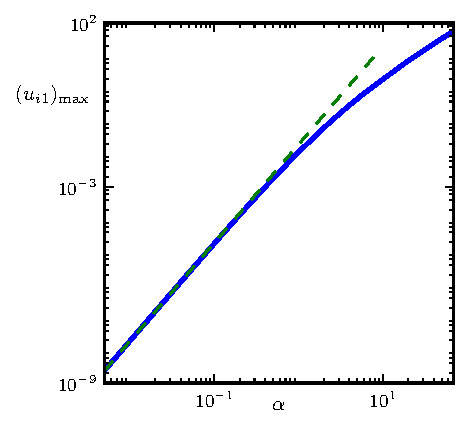
\includegraphics{Fig10}
        \label{fig:profile:qx}
    \end{subfigure}%
    \begin{subfigure}[b]{.5\linewidth}
        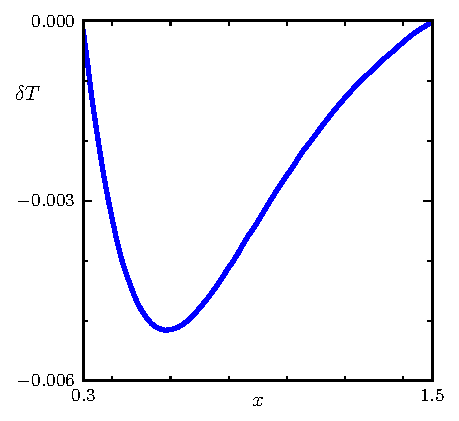
\includegraphics{Fig11}
        \label{fig:profile:qy}
    \end{subfigure}\\[-6pt]
    \begin{subfigure}[b]{.5\linewidth}
        \includegraphics{Fig12}
        \label{fig:profile:P}
    \end{subfigure}%
    \begin{subfigure}[b]{.5\linewidth}
        \includegraphics{Fig13}
        \label{fig:profile:Pyy}
    \end{subfigure}\\[-6pt]
    \begin{subfigure}[b]{.5\linewidth}
        \includegraphics{Fig14}
        \label{fig:profile:Pxx}
    \end{subfigure}%
    \begin{subfigure}[b]{.5\linewidth}
        \includegraphics{Fig15}
        \label{fig:profile:Pzz}
    \end{subfigure}\\[-6pt]
    \phantomcaption
\end{figure}
\begin{figure}
    \ContinuedFloat
    \begin{subfigure}[b]{.5\linewidth}
        \includegraphics{Fig16}
        \label{fig:profile:tau}
    \end{subfigure}%
    \begin{subfigure}[b]{.5\linewidth}
        \includegraphics{Fig17}
        \label{fig:profile:omega}
    \end{subfigure}\\[-12pt]
    \caption{The profiles of the macroscopic variables}
    \label{fig:profiles}
\end{figure}

Fig.~\ref{fig:profiles} shows the profiles of the macroscopic variables.
Note some of their features.
Due to a growth in the gas pressure, the slip of the gas along the plate decreases
with increasing its speed (see also~\eqref{eq:hilbert_boundary_expansion}).
The temperature jump decreases in the same way.
In the linear case, the longitudinal heat-flow vector \(q_x\) is presented only in the Knudsen layer,
but due to the strong anisotropy of the distribution function at large \(\Delta{v}\),
its bulk component increases faster than \((\Delta{v})^2\).
Owing to a significant heating of the gas at large \(\Delta{v}\),
the transverse heat-flow vector \(q_y\) grows faster than \((\Delta{v})^2\) too.
Furthermore, depending on the \(\Delta{v}\) and \(\Kn\), \(q_x\) prevails over \(q_y\) at most.
The longitudinal stress \(P_{xx}\) is always greater than \(P_{yy}\) and \(P_{zz}\).
In the Knudsen layer, for small \(\Kn\), the constant stress \(P_{yy}\) becomes more than \(P_{zz}\).
The temperature of the gas increases with \(\Kn\), because more rarefied gas
has a lower thermal conductivity.

\begin{figure}
    \centering
    \includegraphics{Fig18}
    \caption{The dependence of the shear stress on the Knudsen number}
    \label{fig:shear}
\end{figure}

\begin{figure}
    \centering
    \includegraphics{Fig19}
    \caption{The dependence of the longitudinal mass flow on the Knudsen number}
    \label{fig:flow}
\end{figure}

\begin{figure}
    \centering
    \includegraphics{Fig20}
    \caption{The dependence of the longitudinal heat flow on the Knudsen number}
    \label{fig:qflow}
\end{figure}

\begin{figure}
    \centering
    \includegraphics{Fig21}
    \caption{The dependence of the transverse heat flow on the Knudsen number}
    \label{fig:qflowy}
\end{figure}

\begin{figure}
    \centering
    \includegraphics{Fig22}
    \caption{The dependence of the difference \(P_{xx}-P_{yy}\) on the Knudsen number}
    \label{fig:pxx}
\end{figure}

\begin{figure}
    \centering
    \includegraphics{Fig23}
    \caption{The dependence of the difference \(P_{zz}-P_{yy}\) on the Knudsen number}
    \label{fig:pzz}
\end{figure}

\begin{figure}
    \centering
    \includegraphics{Fig24}
    \caption{The dependence of the temperature distribution on the Knudsen number}
    \label{fig:temp}
\end{figure}

Figs.~\ref{fig:shear}---\ref{fig:temp} show the macroscopic variables,
integrated over half of the volume between the plates, in dependence on the Knudsen number.
To depict the difference between results clearer,
we subtract the asymptotic solutions in two limits: \(\Kn\to0\) and \(\Kn\to\infty\),
and use the logarithmic scale.
Quantities with an asterisk are computed from the Navier--Stokes equations~\eqref{eq:Navier-Stokes}
with the nonslip boundary conditions~\eqref{eq:nonslip_bc}:
\begin{gather*}
    P_{\NS xy}^* = \frac1k \int_0^\frac12 P_{xy} \dd{y}, \quad P_{\NS xy} = P_{\NS xy}^*(\Delta{v}\to0) = -\gamma_1\frac{\Delta{v}}2, \\
    v_{\NS x}^* = \int_0^\frac12 v_x \dd{y}, \quad v_{\NS x} = v_{\NS x}^*(\Delta{v}\to0) = \frac{\Delta{v}}8, \\
    \tau_{\NS}^* = \int_0^\frac12 \tau \dd{y}, \quad
        \tau_{\NS} = \tau_{\NS}^*(\Delta{v}\to0) = \frac{\gamma_1}{\gamma_2}\frac{(\Delta{v})^2}{30}.
\end{gather*}
Their numerical values are shown in Tab.~\ref{table:NS_params}.

\begin{table}
    \centering
    \begin{tabular}{|c|c|c|c|}
        \hline
        \(\Delta{v}\) & \(\displaystyle P_{\NS xy}^*/P_{\NS xy}\) & \(\displaystyle v_{\NS x}^*/v_{\NS x}\) & \(\displaystyle \tau_{\NS}^*/\tau_{\NS}\) \\ \hline
        0.1 & 1.000220 & 0.999945 & 1.000049 \\ \hline
          1 & 1.021740 & 0.994715 & 1.004237 \\ \hline
          2 & 1.083898 & 0.981103 & 1.015173 \\ \hline
          5 & 1.438344 & 0.931106 & 1.055818 \\ \hline
    \end{tabular}
    \caption{Quantities obtained from the numerical solution of the Navier--Stokes equations}
    \label{table:NS_params}
\end{table}

Figs.~\ref{fig:shear}---\ref{fig:qflow} show the macroscopic variables
that are not equal to zero in the linearized problem.
Verification of the results is based on the comparison with the accurate numerical solution
of the linearized Boltzmann equation presented in~\cite{Ohwada1990} (the black line).
For comparison with the solution of the BKW equation (the cyan line),
\(k\) is replaced in~\eqref{eq:bkw_solution} by the following quantities:
\(\gamma_1k\) in Fig.~\ref{fig:shear},~\ref{fig:flow} and \(\gamma_2k\) in Fig.~\ref{fig:qflow}.
With this treatment, the transport coefficients of viscosity and thermal conductivity
for the BKW and hard-sphere models coincide, respectively.
In Fig.~\ref{fig:flow}, the deviation of the main curves (the red line)
from the asymptotic solution for small \(\Kn\) (the blue line) indicates
that the error of the results obtained by the projection method does not exceed \(10^{-3}\).
The DSMC method (the green line) shows a satisfactory accuracy for finite \(\Delta{v}\),
but there are significant fluctuations in the results for \(\Delta{v}=0.1\).
In Fig.~\ref{fig:shear}, the DSMC results differ slightly from the results of the projection method.
This difference vanishes with the time step tending to zero.

Figs.~\ref{fig:qflowy}---\ref{fig:temp} show the macroscopic variables
arising as a square of the \(\Delta{v}\).
Results for \(\Delta{v}=0.1\) are omitted due to low precision.
Taking into account the accuracy of individual approaches,
all presented results are in good agreement.

\section{Concluding remarks}

%%% Asymptotic analysis, its connection to NS equations
In the context of the plane Couette-flow problem,
a comparative analysis of the applied numerical methods can be carried out.
For small \(\Kn\), the asymptotic analysis of the Boltzmann equation has demonstrated
its superiority in terms of accuracy and efficiency.
The derived fluid-dynamic-type equations, coinciding with the Navier--Stokes equations,
with the appropriate slip boundary conditions allow to obtain
the distribution of the macroscopic variables with an error \(\mathcal{O}(\Kn^2)\).
Note that the expressions for the stress tensor and heat-flow vector
differ from the Newton's and Fourier's laws.
However, in the general case, firstly, the expansion parameter in the viscous boundary layer
is \(\sqrt\Kn\) (in contrast to \(\Kn\)), and, secondly,
the asymptotic analysis in curvilinear coordinates leads to the cumbersome expressions~\cite{Sone2002}.
In addition, if the viscous layer is not smooth,
the method of constructing the asymptotic solutions are not obvious~\cite{Aoki2014}.

%%% Accuracy of the projection method vs DSMC
By means of the direct numerical solution of the Boltzmann equation using the projection method,
an error less \(10^{-3}\) has been achieved for a wide range of the external parameters:
\(0.01 \le \Kn \le 100\) and \(0.1 \le \Delta{v} \le 5\).
The main restriction to obtain a high-accuracy solution,
is the problem of selecting the appropriate discretization of velocity space
to provide a satisfactory approximation of the distribution function.
This problem is typical for discrete-velocity methods.
The high performance of the projection method (as well as any disrete-velocity method)
stems from the fact that the velocity grid is the same in the whole volume occupied by the gas.
Therefore, for problems with a finite curvature of the boundary surface,
it is necessary to use a uniform velocity grid, which fails to approximate
the large gradients of the distribution function in the Knudsen layer accurately.
Statistical modeling techniques do not have such complications.
The DSMC method, as expected, demonstrates his versatility,
but fails to obtain sufficiently accurate results
due to the typical statistical fluctuations, especially for small \(\Delta{v}\).

%%% Computational load and perspectives
In the present paper, a direct numerical solution of the Boltzmann equation, on average,
took an order of magnitude more time than the statistical modeling.
In comparison between computational loads, the DSMC method has an advantage for large \(\Kn\),
but is known to require a significant increase in simulation time for small \(\Kn\).
In view of the above discussion, the projection method on nonuniform grids can be recommended
as a precision tool for solving the Boltzmann equation with arbitrary Knudsen and Mach numbers,
but for boundary-value problems with a simple rectangular geometry.

\appendix
\section{The transport coefficients \(\gamma_8\), \(\gamma_9\) and \(\gamma_{10}\)}
\label{sec:gamma_coeffs}

The general formulas for calculation \(\gamma_8\), \(\gamma_9\) and \(\gamma_{10}\)
for hard-sphere molecules are taken from~\cite{Sone2000, Sone2002, Sone2007}:
\begin{gather}
    \gamma_8 = I_6\left(\Q_2 - \QQ_{22}\right) + \frac17 I_8\left(\Q_3 - \QQ_3\right), \label{eq:gamma_8}\\
    \gamma_9 = -I_6\left(\B\right), \label{eq:gamma_9}\\
    \gamma_{10} = \frac58 I_6\left(\T{1}_1 + \T{2}_1 - 2\TT_{12}\right)
        + \frac18 I_8\left(\T{1}_2 + \T{2}_2 - 2\TT_2\right). \label{eq:gamma_10}
\end{gather}
Here,
\begin{equation}\label{eq:I_n}
    I_n[Z(\zeta)] = \frac{8}{15\sqrt\pi} \int_0^\infty \zeta^n Z(\zeta) \exp(-\zeta^2) \dd\zeta,
\end{equation}
and the integrands can be obtained from the corresponding integral equations:
\begin{align}
    \mathcal{L}\left(\zeta_x\mathcal{A}\right) &= -\zeta_x\left(\zeta^2-\frac52\right), \label{eq:A}\\
    \mathcal{L}\left(\zeta_x\zeta_y\mathcal{B}\right) &= -2\zeta_x\zeta_y, \label{eq:B}\\
    \mathcal{L}\left(\zeta_x\zeta_y\B\right) &= \zeta_x\zeta_y\mathcal{B}, \label{eq:B_4}
\end{align}
\begin{align}
    \mathcal{L}\left( \zeta_x\zeta_y\zeta_z\T{1}_2 \right)
        &= -\zeta_x\zeta_y\zeta_z\left(2\mathcal{A} - \frac1\zeta\der[\mathcal{A}]{\zeta}\right), \label{eq:T2a}\\
    \mathcal{L}\left[ \zeta_x\left(3\T{1}_1 + \zeta_x^2\T{1}_2\right) \right]
        &= -\zeta_x^3\left(2\mathcal{A} - \frac1\zeta\der[\mathcal{A}]{\zeta}\right), \label{eq:T1a}\\
    \mathcal{L}\left( \zeta_x\zeta_y\zeta_z\T{2}_2 \right)
        &= -\zeta_x\zeta_y\zeta_z\left((\zeta^2-3)\mathcal{B} - \frac\zeta2\der[\mathcal{B}]{\zeta}\right), \label{eq:T2b}\\
    \mathcal{L}\left[ \zeta_x\left(3\T{2}_1 + \zeta_x^2\T{2}_2\right) \right]
        &= -\zeta_x^3\left((\zeta^2-3)\mathcal{B} - \frac\zeta2\der[\mathcal{B}]{\zeta}\right) + \frac{3\gamma_1}{2}\zeta_x, \label{eq:T1b}\\
    \mathcal{L}\left( \zeta_x\zeta_y\zeta_z\TT_2 \right)
    	&= \mathcal{J}\left( \zeta_x\mathcal{A}, \zeta_y\zeta_z\mathcal{B} \right), \label{eq:TT2}\\
    \mathcal{L}\left[ \zeta_y\left(\TT_{12} + \zeta_x^2\TT_2\right) \right]
        &= \mathcal{J}\left( \zeta_x\mathcal{A}, \zeta_x\zeta_y\mathcal{B} \right), \label{eq:TT12}
\end{align}
\begin{align}
    \mathcal{L}\left[ \zeta_x\zeta_y \left( 3\zeta_z^2-\zeta_x^2 \right)\Q_3 \right]
        &= -\zeta_x\zeta_y\left( 3\zeta_z^2-\zeta_x^2 \right)\left(2\mathcal{B} - \frac1\zeta\der[\mathcal{B}]{\zeta}\right), \label{eq:Q3}\\
    \mathcal{L}\left[ \zeta_x\zeta_y \left( 3\Q_2+\zeta_x^2\Q_3 \right) \right]
        &= -\zeta_x^3\zeta_y\left(2\mathcal{B} - \frac1\zeta\der[\mathcal{B}]{\zeta}\right), \label{eq:Q2}\\
    \mathcal{L}\left[ \zeta_x\zeta_y\left( 3\zeta_z^2 - \zeta_x^2 \right)\QQ_3 \right]
        &= \mathcal{J}\left( \zeta_x\zeta_y\mathcal{B}, \zeta_z^2\mathcal{B} \right)
        + 2\mathcal{J}\left( \zeta_x\zeta_y\mathcal{B}, \zeta_x\zeta_z\mathcal{B} \right)
        - \mathcal{J}\left( \zeta_x\zeta_y\mathcal{B}, \zeta_x^2\mathcal{B} \right), \label{eq:QQ3}\\
    \mathcal{L}\left[ \zeta_x\zeta_y \left( \QQ_{22} + \zeta_z^2\QQ_3 \right) \right]
        &= \mathcal{J}\left( \zeta_x\zeta_y\mathcal{B}, \zeta_x\zeta_z\mathcal{B} \right) \label{eq:QQ2}
\end{align}
with subsidiary conditions for \(\mathcal{A}\), \(\T{m}_1\), \(\TT_{12}\):
\begin{gather}
    \int_0^\infty \zeta^4 \mathcal{A} E \dd\zeta = 0, \label{eq:A_constraint}\\
    \int_0^\infty \left( 5\zeta^4\T{m}_1 + \zeta^6\T{m}_2 \right) E \dd\zeta = 0, \label{eq:Tm_constraint}\\
    \int_0^\infty \left( 5\zeta^4\TT_{12} + \zeta^6\TT_2 \right) E \dd\zeta = 0, \label{eq:T12_constraint}
\end{gather}
Collision operators \(\mathcal{L}\) and \(\mathcal{J}\) are related to the collision integral \(J\) as follows:
\begin{equation}\label{eq:mathcalLJ}
    E\mathcal{L}(\phi) = 2J(1, E\phi), \quad E\mathcal{J}(\phi, \psi) = J(E\phi, E\psi).
\end{equation}

The integral equations~\eqref{eq:A}--\eqref{eq:B} are solved accurately in~\cite{Pekeris1957}
by reducing them to ordinary differential equations.
Another example of reduction for computation \(\gamma_3\) can be found in~\cite{Ohwada1992}.
For present paper, the integral equations in question are solved
by the simple iterative method and direct quasi-Monte Carlo integration.
The desired functions are shown in Fig.~\ref{fig:transport_functions}.

\begin{figure}
    \centering
    \begin{subfigure}[b]{0.33\textwidth}
        \includegraphics[right]{Fig25}
        \label{fig:B}
    \end{subfigure}%
    \begin{subfigure}[b]{0.33\textwidth}
        \includegraphics[right]{Fig26}
        \label{fig:B_4}
    \end{subfigure}%
    \begin{subfigure}[b]{0.33\textwidth}
        \includegraphics[right]{Fig27}
        \label{fig:T1_1}
    \end{subfigure}\\[-6pt]
    \begin{subfigure}[b]{0.33\textwidth}
        \includegraphics[right]{Fig28}
        \label{fig:T1_2}
    \end{subfigure}%
    \begin{subfigure}[b]{0.33\textwidth}
        \includegraphics[right]{Fig29}
        \label{fig:T2_1}
    \end{subfigure}%
    \begin{subfigure}[b]{0.33\textwidth}
        \includegraphics[right]{Fig30}
        \label{fig:T2_2}
    \end{subfigure}\\[-6pt]
    \begin{subfigure}[b]{0.33\textwidth}
        \includegraphics[right]{Fig31}
        \label{fig:TT12}
    \end{subfigure}%
    \begin{subfigure}[b]{0.33\textwidth}
        \includegraphics[right]{Fig32}
        \label{fig:TT2}
    \end{subfigure}%
    \begin{subfigure}[b]{0.33\textwidth}
        \includegraphics[right]{Fig33}
        \label{fig:Q2}
    \end{subfigure}\\[-6pt]
    \begin{subfigure}[b]{0.33\textwidth}
        \includegraphics[right]{Fig34}
        \label{fig:Q3}
    \end{subfigure}%
    \begin{subfigure}[b]{0.33\textwidth}
        \includegraphics[right]{Fig35}
        \label{fig:QQ22}
    \end{subfigure}%
    \begin{subfigure}[b]{0.33\textwidth}
        \includegraphics[right]{Fig36}
        \label{fig:QQ3}
    \end{subfigure}\\[-6pt]
    \caption{The transport functions for hard-sphere molecules}
    \label{fig:transport_functions}
\end{figure}


\bibliographystyle{spmpsci} % spbasic, spmpsci, spphys
\bibliography{springer}

\end{document}

